\section{Preprocessing Data}
\label{cha:preprocessing}

In total, two datasets were used to create features for testing the different classifiers:
\textit{movies\_metadata.csv} and \textit{credits.csv}. The dataset \textit{movies\_metadata.csv} contains 45,463 rows and 23 columns excluding the id-column. The dataset \textit{credits.csv} contains 45,463 rows and 2 columns excluding the id-column.

\paragraph{Vertical scaling}
Both dimensions of the dataset \textit{movies\_metadata.csv} were processed. 
The columns \textit{revenue} and \textit{budget} are the major components for this project, since they are used to derive the label values for the training instances. Because of the described inconsistencies of both attributes throughout the dataset, new and reliable values need to be assigned to both of them. To achieve this, two parsers were programmed to mine the financial information for all movies contained in the dataset. One parser extracted the values from the \textit{IMDb}\footnote{\hyperref{http://www.imdb.com/}{external_sources}{ref:IMDB}{The IMDB database: http://www.imdb.com/}} website and a second parser extracted the values from the \textit{The Numbers}\footnote{\hyperref{http://www.the-numbers.com/research-analysis}{external_sources}{ref:numbers}{the numbers website: http://www.the-numbers.com/research-analysis}} website. With these approaches it was possible to gain consistent and comparable values for \textit{budget} and \textit{revenue}. Records containing missing values as well as duplicates of records contained in the raw data were identified and discarded. The resulting final vertical size of the dataset is 3,913 records.

%The revenue and budget played a major role for the data mining task. Therefore all datasets without information on each column had to be dropped, which was a major part of the dataset. Also duplicates were identified and discarded. 
 
%After this, the dataset shrunk to roughly 4,000 rows. To retain some numbers and still use datasets which had only missing out revenue or budget two approaches were implemented: A parser for the IMDB database\footnote{
%\hyperref{http://www.imdb.com/}{external_sources}{ref:IMDB}{The IMDB database: http://www.imdb.com/}} API and for the The Numbers\footnote{\hyperref{http://www.the-numbers.com/research-analysis}{external_sources}{ref:numbers}{the numbers website: http://www.the-numbers.com/research-analysis}} API was programmed and run. With these approaches it was possible to gain the real values of budget and revenue for the dataset. By mining two of the most reliable movie-datasources out in the web, it was also possible to determine rows, which used foreign currency values in their revenue or only revenue based on the local market (e.g. only in the US).

\paragraph{Horizontal scaling}
\begin{wrapfigure}{r}{0.6\textwidth}
	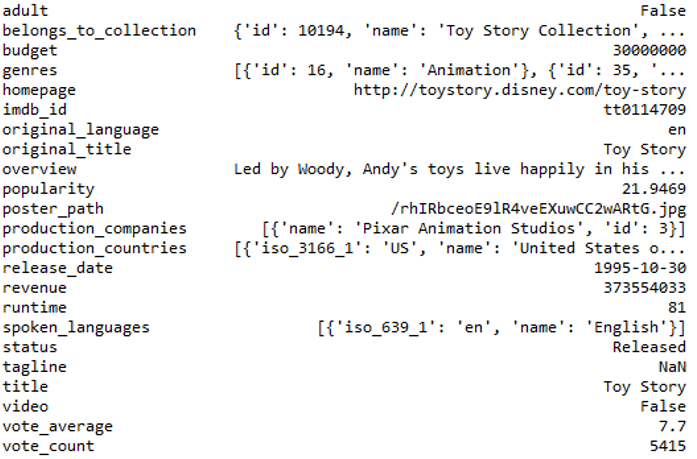
\includegraphics[width=0.6 \textwidth]{images/3_metadata_columns.png}
	\caption{Remained columns of \textit{movies\_metadata.csv} are highlighted in yellow}
	\label{img:mm_columns}
\end{wrapfigure}

Based on the assumptions that budget and revenue are crucial numbers, also other features have been selected for the modeling. A special focus is placed on the following data columns: the release year, the genre, the production country as well as the production company, the spoken languages, the runtime and the fact whether a movie belongs to a collection or not. Due to high encoding effort for these features, further columns are not taken into account during this project. Figure \ref{img:mm_columns} gives an overview on which information was retained.

The reason why information, which could have been potentially interesting, had to be dropped, was mainly for time reasons. Preprocessing took about 70\% of the projects time period\footnote{Mainly due to the fact that heaps of problems arose from the dataset, which can be read in chapter \ref{cha:data_selection}.}. Thus, the team was able to focus on preprocessing of mentioned columns. Prospects of additional applications and improvements can be found in later paragraphs.

After dropping not selected features, eleven columns remain. Combined with the two columns from the \textit{credits.csv} dataset, thirteen columns are used as a basis to create features for finding the best performing classifiers.

In order to transform the data into a suitable representation for forecasting a movie's success, preprocessing has been mandatory. For each column zero or more preprocessing steps from the following list were performed: \textit{Merging of columns, discretization (binning) of features, extracting information out of columns, one hot encoding, normalizing.}

The following sections explain the preprocessing in more detail. Figure \ref{img:features} shows precisely, which operations were executed on each column and how the data types changed.
\begin{figure}[h]
	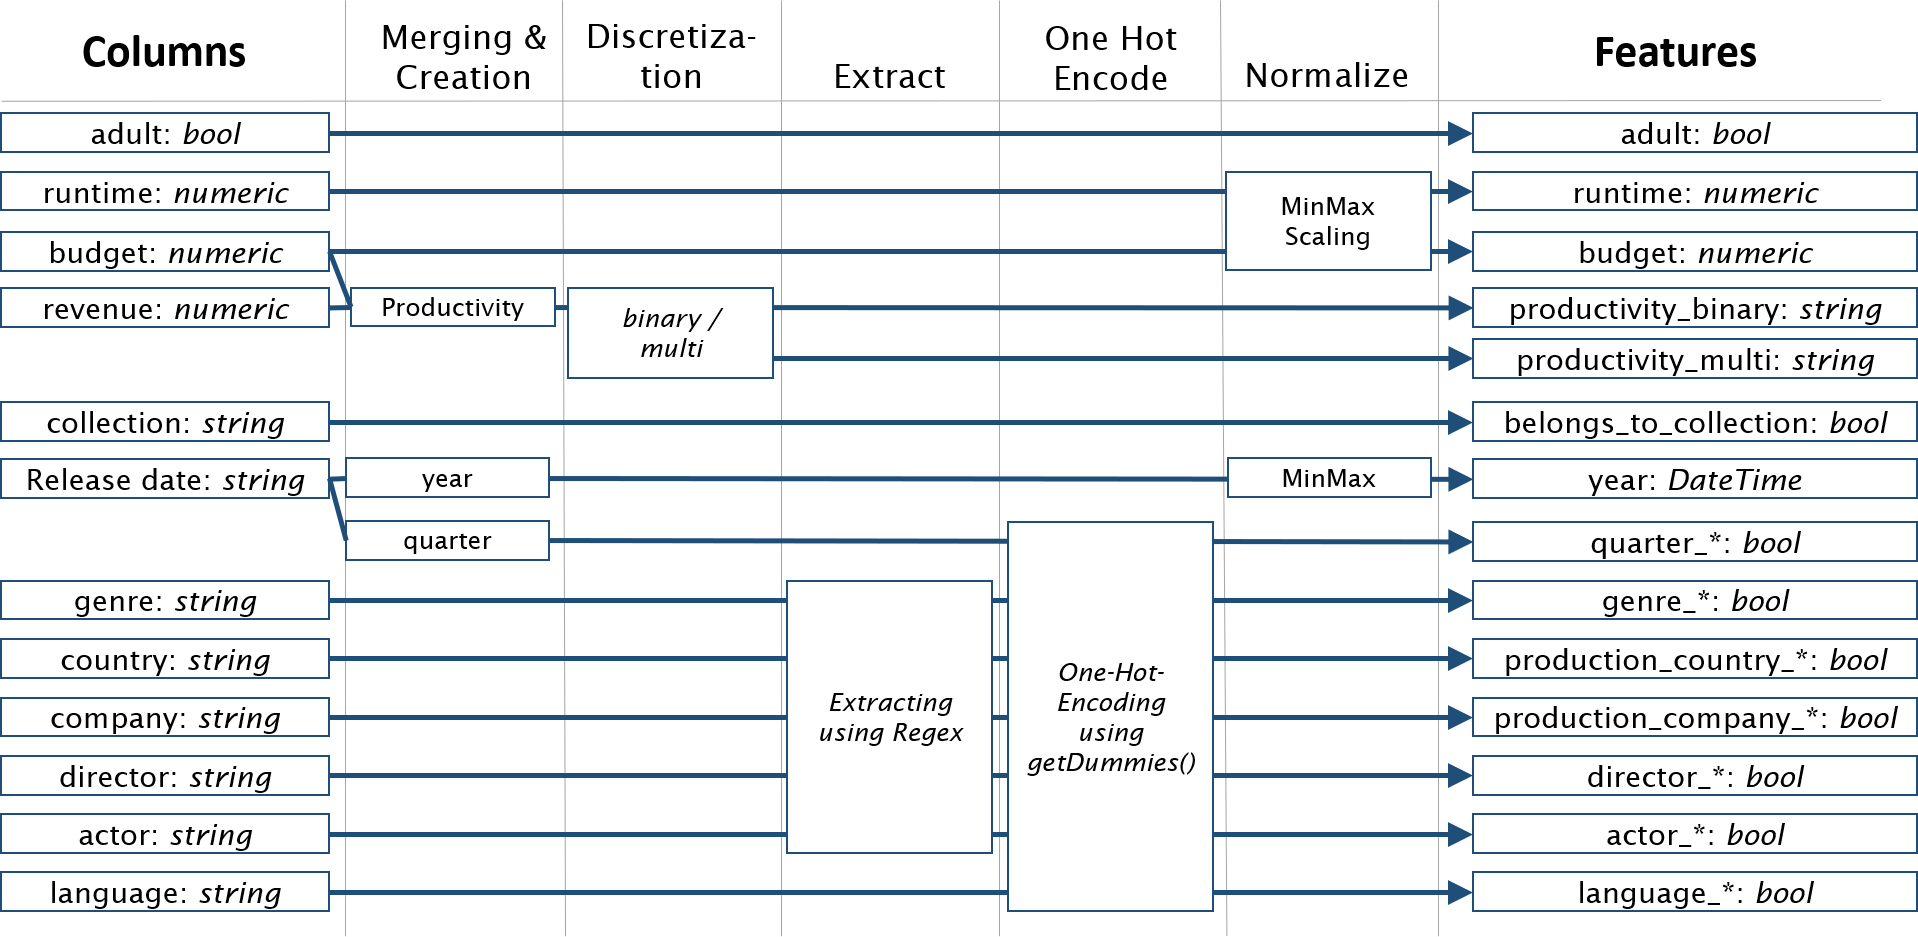
\includegraphics[width=\textwidth]{images/3_features.png}
	\caption{Features created during preprocessing}
	\label{img:features}
\end{figure}
\FloatBarrier

\paragraph{Merging and creating columns.}
\label{sec:merge_create}
When a new movie is planned, the finances are one of the most important concerns. As described in chapter \ref{sec:data_exploration}, a new column had to be introduced, namely the productivity.
%It is a quotient, computed by dividing revenue through budget. If the productivity is higher than one, the movie derives profit, if the productivity is less than one, the movie derives a loss. That way, above mentioned issues can be avoided.
The column revenue was dropped afterwards.

Considering the release date of a movie, the assumption was made that the demand for movies is higher in quarter four of the year (time of winter and christmas). This was confirmed by checking the numbers\footnote{Check for details on revenues in video-selling:\\ \hyperref{https://de.statista.com/statistik/daten/studie/182319/umfrage/umsatzentwicklung-im-video-kaufmarkt-quartalszahlen/}{link}{Statista revenue movies}{https://de.statista.com/statistik/daten/studie/182319/umfrage/umsatzentwicklung-im-video-kaufmarkt-quartalszahlen/}}. Hence, two new columns containing the release quarter and the release year have been created. The column release year has been dropped afterwards.

\paragraph{Discretization}
During this preprocessing step, the created column containing the continuous attribute \textit{productivity} was binned using a binary and a multi-way split. The multi-way split contains four bins of user-provided boundaries ranging from $[0.0, 1.00)$ labeled \textit{unproductive}, $[1.0, 2.00)$ labeled \textit{smallProductivity}, $[2.0, 5.00)$ labeled \textit{goodProductivity} and $[5.0, \infty)$ labeled \textit{highProductivity}. The binary split was implemented using user-provided boundaries ranging from $[0.0, 1.0)$ labeled \textit{no} and $[1.0, \infty)$ labeled \textit{yes}. For each bin a new column was added (\textit{productivity\_binned\_multi}, \textit{productivity\_binned\_binary}) and the continuous attribute \textit{productivity} was dropped.

\paragraph{Extracting information}
Some information, including the production companies, actors and crew members are provided as a JSON Object inside a column of the dataset. The first approach, parsing  JSON data failed, because  some columns contained invalid JSON format. After a closer analysis of the values inside the column, a new extraction concept could be developed. Given the values of the cast column, actors could be extracted by looking for the regular expressions inside the correlating values. For example actors could be identified by looking for the parameter name, and extracting the value provided by the parameter. The same procedure with slight changes has been applied to the extraction of the directors and the countries of production.

After evaluation of the extracted parameters, ambiguous names for the production companies have been discovered. For example: "Twenty Century Fox", "Twenty Century-Fox" and "Twenty Century Fox Production". Without any further preprocessing each of the values would be one hot encoded separately. Therefore additional preprocessing has been performed to remove different ways of writing the same company, and therefore providing the same textual values for one hot encoding.

\paragraph{Normalizing, thresholding and one hot encoding}
The extracted information genre, production country, production company director, original language  and actor were one hot encoded using the pandas \textit{get\_dummies()}\footnote{The \hyperref{https://pandas.pydata.org/pandas-docs/stable/generated/pandas.get_dummies.html}{documentation}{pd.getDumies}{Documentation on pandas \textit{get\_dummies()} function can be found online}} function. After one-hot-encoding, the dataset consisted of about 49,000 columns\footnote{The high number is due to the high number of different actors, directors, production companies and production countries.}.


In order to reduce the amount of columns and to filter out unnecessary data a threshold can be applied to each classifier, as described in chapter \ref{cha:data_mining}. To create equal importance among the different numeric values in the data set, these columns (including runtime, budget and year) are normalized using MinMax scaling.




%\begin{itemize}
%	\item Transform data into a representation that is suitable for the chosen data mining methods
%	\begin{itemize}
%		\item number of dimensions
%		\item scales of attributes (nominal, ordinal, numeric)
%		\item amount of data (determines hardware requirements)
%	\end{itemize}
%	\item Methods
%	\begin{itemize}
%		\item Aggregation, sampling
%		\item Dimensionality reduction / feature subset selection
%		\item Attribute transformation / text to term vector
%		\item Discretization and binarization
%	\end{itemize}
%	\item Good data preparation is key to producing valid and reliable models
%	\item Data preparation estimated to take 70-80\% of the time and effort of a data mining project!
%\end{itemize}

%\section{A list of problems we encountered}
%\begin{enumerate}
%	\item \textbf{list further problems we had and solved!}
%	\item Prod. Comp.: Same prod. company named differently -> using Regex to solve (Steffen)
%	\item dataset: 5 datasets have duplicates
%\end{enumerate}
